%===================================================================================================
% システム設計
%===================================================================================================
\chapter{システム設計}
第I部では,ユーザの音声と視線方向を利用した指示理解をテーマとし,システムの構築を行う.
本章では,設計するシステムの概要,音声認識,物品情報の取得,対象物品の推定法について述べる.

%---------------------------------------------------------------------------------------------------
\section{概要}
本システムの目的は,ユーザの発する音声内容を基に,環境内の複数候補から対象物品を推定することである.
ここでは,複数候補から選定するためのアプローチとして視野方向を利用し,指示発出時に注視している物品をユーザの意図する対象と仮定する.

目的の実現にあたっては,次の3つの環境情報を利用する.
1つ目は,ユーザの発する音声指示である.
本システムでは,サービスを開始するためのトリガとして,入力された音声を認識し,文字列に起こす.
2つ目は,物品情報である.
認識した音声内容に従って,物品情報データベースを照会し,物品候補の位置情報を取得する.
3つ目は,ユーザの視野方向である.
計測される視野の方向と候補物品の位置から,注視している可能性の高い物品を決定する.本システムでは,まず,視野方向がより正確な指示理解に寄与しうることを確認するために,モーションキャプチャーシステムにより眼鏡の位置・姿勢を計測し,1人称画像の代用とした.
しかし,最終的に1人称画像を利用するに至らず,第II部に述べるシステムの構築に移行した.

システムはTMSでの稼働を想定し,各プロセスの記述と通信のフレームワークとしてRobot Operating System (ROS)\footnote{http://www.ros.org/}を利用した.
次節より,各要素の実装内容について述べる.

%---------------------------------------------------------------------------------------------------
\section{音声指示の認識}
音声の認識には,オープンソースの連続音声認識エンジンJulius\footnote{http://julius.sourceforge.jp}を利用した.
juliusの認識プロセスを図{\ref{fig:julius}}に示す.
julius単体は,入力音声から単語列を探索するための基本的なモジュールを構成している.
音声認識システムとして実際に稼働するためには,julius本体に付随して,語彙と各単語の発音を規定する単語辞書,各単語間の確率的な連鎖関係を規定する言語モデル,各単語の音声波形を統計的にモデル化した音響モデルを要する.
juliusの最大の特徴として,このようなモデルやパラメータを自由に設定することができ,自由度・汎用性が非常に高いことが挙げられるが,その学習には膨大なデータと時間を要する.そのため,本研究では,予め標準的なパラメータを設定したディクテーション実行キットを利用する.
音声入力デバイスとして,図{\ref{fig:headset}}のヘッドセットを用いた.
%
\begin{figure}[htbp]
\begin{tabular}{cc}
%
  \begin{minipage}{0.55\textwidth}
    \begin{center}
      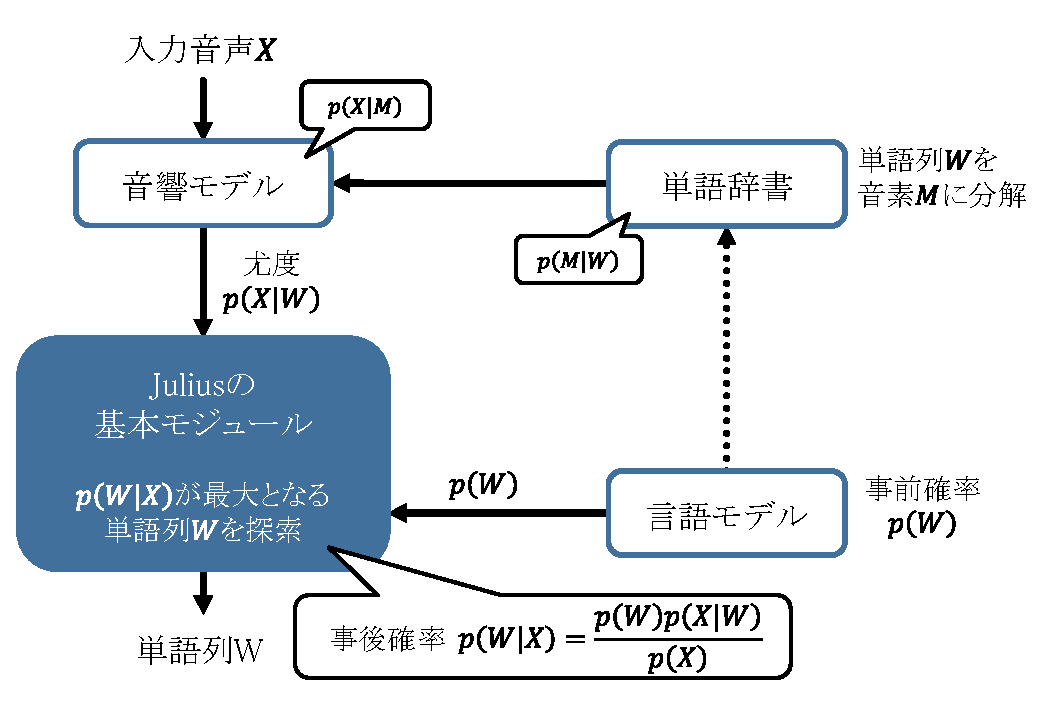
\includegraphics[height=60mm]{figure/julius.eps}
      \vspace{-10mm}
      \caption{juliusの認識プロセス}
      \label{fig:julius}
    \end{center}
  \end{minipage}
%
  \begin{minipage}{0.4\textwidth}
    \begin{center}
      
\includegraphics[height=80mm]{figure/headset.eps}
      \vspace{-20mm}
      \caption{ヘッドセット}
      \label{fig:headset}
    \end{center}
  \end{minipage}
%
\end{tabular}
\end{figure}

%---------------------------------------------------------------------------------------------------
\section{物品情報の取得}
Juliusで認識した音声内容を基に,TMSデータベースを参照し,物品位置情報を取得する.
まず,特定の音声内容とそれに関連する物品IDを結びつけたテーブルを参照し,認識した音声内容が,いずれかに適合すれば,対応する物品IDのリストを作成する.
さらに,そのリストに従って,TMSデータベースにクエリを送信し,各物品の位置情報を取得する.

%---------------------------------------------------------------------------------------------------
\section{指示対象の推定法}
本節では,視野方向を利用して,複数候補から指示対象物品を推定する方法について述べる.
ここでは,計測される眼鏡の正面方向を,ユーザの視野方向と定義する.また,物品までの直線距離と視野方向に対する広がりを評価し,評価値に基づいた候補物品のソーティングを考える.
図{\ref{fig:estimation}}に,概要図を示す.

まず,計測される眼鏡のローカル座標系を視点座標系として定義し,視点座標系から観測した場合の各候補物品の位置ベクトル$ \bm{r}_v $を求める.
さらに,各位置ベクトルの大きさ$ l $と,上述した視野方向との偏角$ \theta $から求まる次式を,物品の評価値$ k $とする.
%
\begin{equation}
\label{eq:sort_key}
{
  k = l (\theta + \theta_{c})
}
\end{equation}

(\ref{eq:sort_key})は,定数$ \theta_{c} $を無視すれば,視野方向直線に対する円弧の長さを表す.
$ \theta_{c} $は,複数候補が視野方向の直線上に並んだ場合に,$ k $が同値となることを避けるために付与した.
すなわち,評価値$ k $が小さい物品ほど,ユーザの位置に近く,視野内の中心に存在する可能性が高い.
視野前方の評価値の分布は,図{\ref{fig:sort_key}}のようになる.
%
\begin{figure}[htbp]
  \vspace{-3mm}
  \begin{center}
    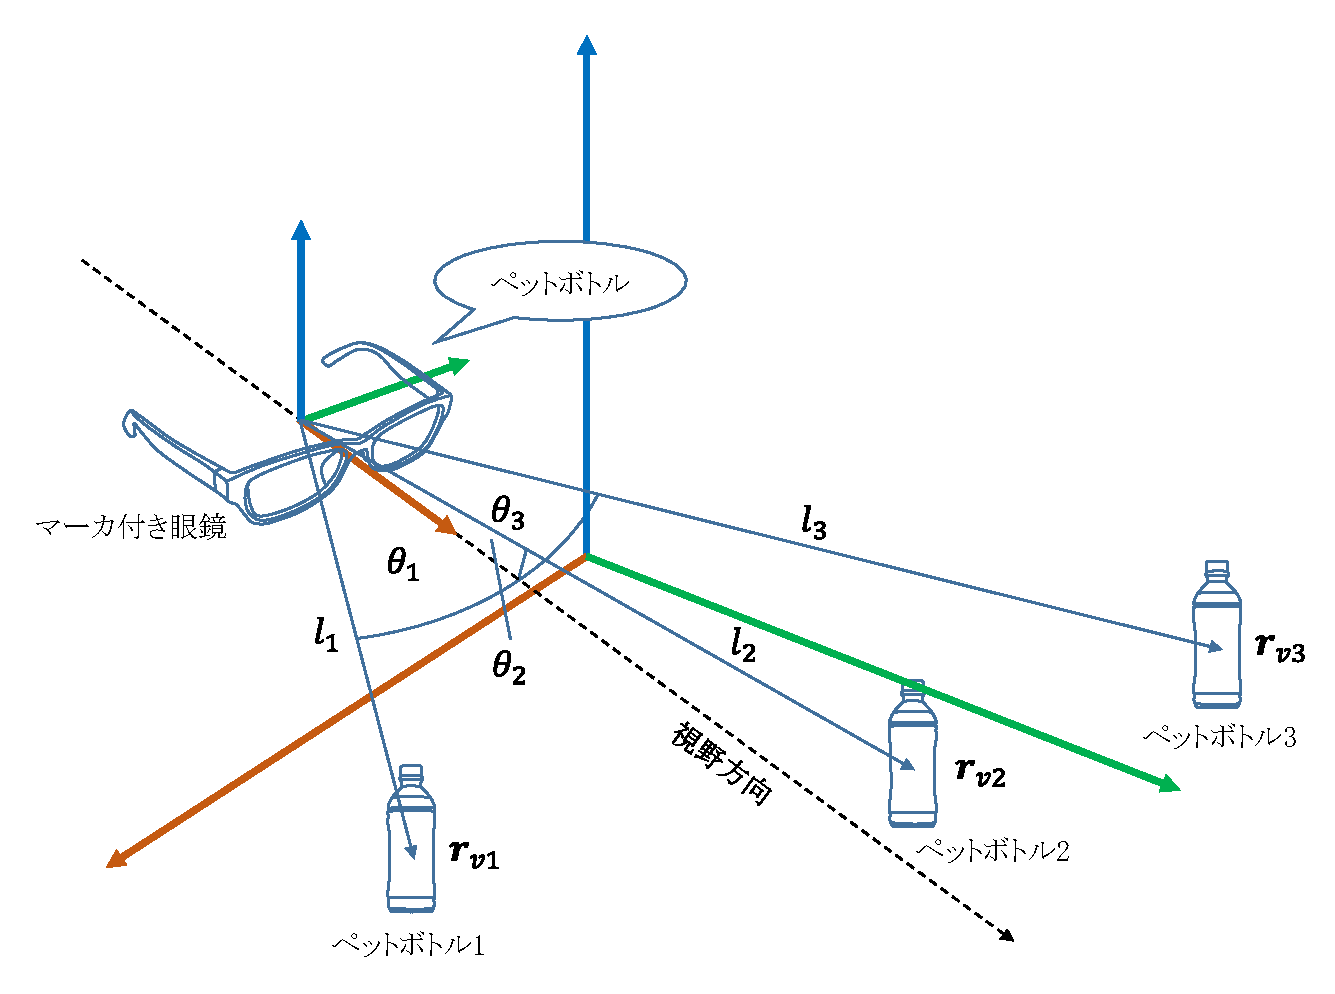
\includegraphics[height=100mm]{figure/estimation.eps}
    \vspace{-5mm}
    \caption{指示対象の推定法}
    \label{fig:estimation}
  \end{center}
\end{figure}
%
\begin{figure}[htbp]
\begin{tabular}{cc}
%
  \begin{minipage}{0.8\textwidth}
    \begin{center}
      \includegraphics[height=70mm]{figure/sort_key.eps}
    \end{center}
  \end{minipage}
%
  \begin{minipage}{0.1\textwidth}
    \begin{center}
      \includegraphics[height=60mm]{figure/sort_key_legends.eps}
    \end{center}
    \vspace{3mm}
  \end{minipage}
%
\end{tabular}
\caption{視野前方の評価値分布}
\label{fig:sort_key}
\end{figure}


\newpage
まず,視点座標系から観測した場合の物品の位置ベクトル$ \bm{r}_v $を求める.
視点座標系を定義するための眼鏡の位置・姿勢の計測には,光学式モーションキャプチャシステムを利用した.
モーションキャプチャのカメラには,Vicon社のBonitaを利用し,計測データの処理とマーカモデル作成を同社のソフトウェアTracker上で行う.
計測対象の眼鏡には,検出のための赤外線反射マーカを4個取り付け,ワールド座標上の3次元点座標とロール角$ \alpha $,ピッチ角$ \beta $,ヨー角$ \gamma $を計測する.
なお,初期状態では,空間内の物体はx軸を正面方向に,z軸を鉛直上方に取る.
図{\ref{fig:coodinates_definition}}に座標系の定義を,図{\ref{fig:glasses_with_markers}}に計測対象とする眼鏡の外観を示す.
%
\begin{figure}[htbp]
\begin{tabular}{cc}
%
  \begin{minipage}{0.5\textwidth}
    \begin{center}
      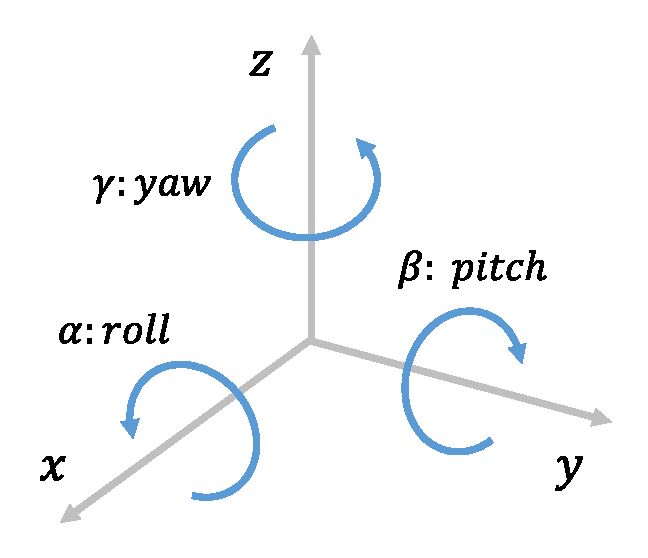
\includegraphics[height=40mm]{figure/coodinates_definition.eps}
      \vspace{-5mm}
      \caption{座標系定義}
      \label{fig:coodinates_definition}
    \end{center}
  \end{minipage}
%
  \begin{minipage}{0.5\textwidth}
    \begin{center}
      \includegraphics[height=40mm]{figure/glasses_with_markers.eps}
      \vspace{-5mm}
      \caption{赤外線反射マーカ付き眼鏡}
      \label{fig:glasses_with_markers}
    \end{center}
  \end{minipage}
%
\end{tabular}
\end{figure}
%

計測される位置・姿勢情報から,ワールド座標系に対する視点座標系の回転行列$ \bm{R} $と並進ベクトル$ \bm{t} $を求める.
ワールド座標系からローカル座標系への変換は,各主軸に関してx-y-zの順に回転を行い,平行移動することで求まるが,ここでは視線方向のみを考えればよいため,x軸(眼鏡正面方向)に関する回転を無視する.
従って,回転行列$ \bm{R} $は,z軸に関する回転行列$ \bm{R}(\gamma) $と,y軸に関する回転行列$ \bm{R}(\beta) $を用いて次式で表す.

\begin{equation}
{
  \bm{R}
  = \bm{R}(\gamma)\bm{R}(\beta)
  = \left(
    \begin{array}{ccc}
      \cos{\gamma} & -\sin{\gamma} & 0 \\
      \sin{\gamma} & \cos{\gamma} & 0 \\
      0 & 0 & 1 \\
    \end{array}
  \right)
  \left(
    \begin{array}{cccc}
      \cos{\beta} & 0 & -\sin{\beta} \\
      0 & 1 & 0 \\
      \sin{\beta} & 0 & \cos{\beta} \\
    \end{array}
  \right)
}
\end{equation}

また,並進ベクトル$ \bm{t} $は眼鏡の3次元位置座標$ (t_x, t_y, t_z) $を用いて,次式で表される.
%
\begin{equation}
{
  \bm{t}
  = \left(
    \begin{array}{ccc}
      t_x & t_y & t_z \\
    \end{array}
  \right)^{\mathrm{T}}
}
\end{equation}
%

これらを用いると,ワールド座標系における物品位置$ \bm{r}_w = \left( x_w, y_w, z_w \right)^{\mathrm{T}} $は,次式によって視点座標系における物品位置$ \bm{r}_v = \left( x_v, y_v, z_v \right)^{\mathrm{T}}$に変換される.
%
\begin{equation}
{
  \bm{r}_v
  = \bm{R}^{\mathrm{T}}\left(\bm{r}_w-\bm{t}\right)
}
\end{equation}
%
\begin{equation}
{
  \left(
    \begin{array}{c}
      x_v \\ y_v \\ z_v \\
    \end{array}
  \right)
  = \left(
    \begin{array}{ccc}
      \cos{\beta}\cos{\gamma} & \cos{\beta}\sin{\gamma} & \sin{\beta} \\
      -\sin{\gamma} & \cos{\gamma} & 0 \\
      -\sin{\beta}\cos{\gamma} & -\sin{\beta}\sin{\gamma} & \cos{\beta} \\
    \end{array}
  \right)
  \left(
    \begin{array}{c}
      x_w - t_x \\ y_w - t_y \\ z_w - t_z\\
    \end{array}
  \right)
}
\end{equation}
%
\begin{figure}[htbp]
\begin{tabular}{cc}
%
  \begin{minipage}{0.5\textwidth}
    \begin{center}
      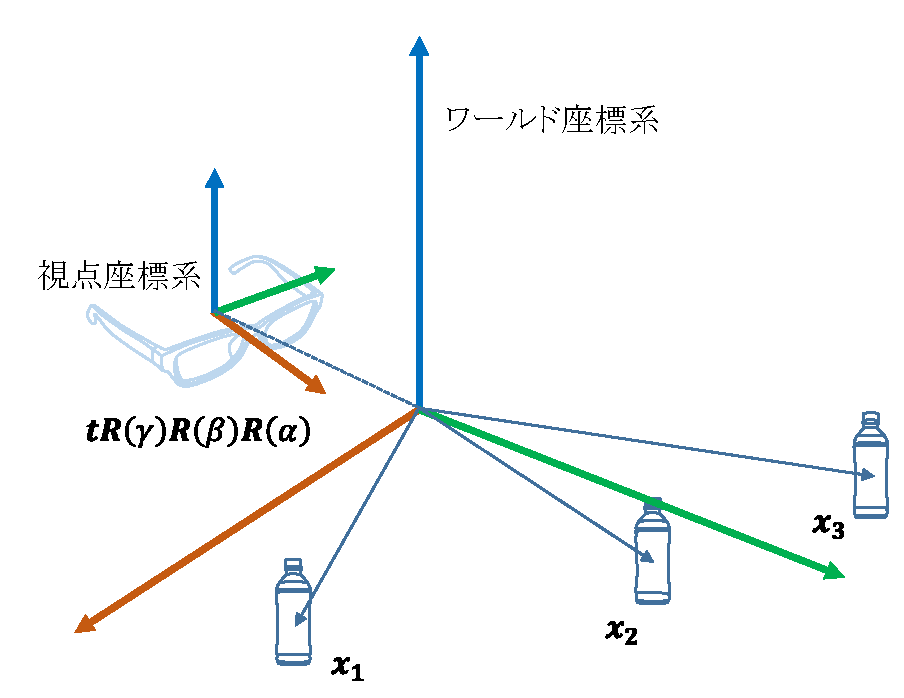
\includegraphics[height=50mm]{figure/world_coodinates.eps}
      \caption{ワールド座標系から観測した各物体位置}
      \label{fig:world_coodinates}
    \end{center}
  \end{minipage}
%
  \begin{minipage}{0.5\textwidth}
    \begin{center}
      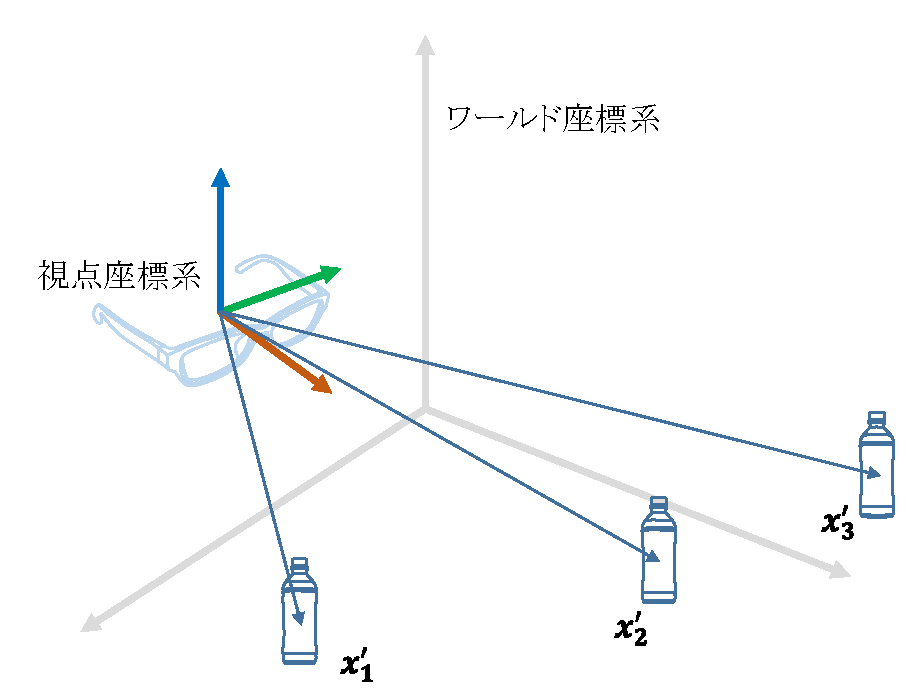
\includegraphics[height=50mm]{figure/view_coodinates.eps}
      \caption{視点座標系から観測した各物体位置}
      \label{fig:view_coodinates}
    \end{center}
  \end{minipage}
%
\end{tabular}
\end{figure}

従って,眼鏡から各物品までの直線距離$ l $は,ベクトル$ \bm{r}_v $の大きさで表される.
%
\begin{equation}
{
  l = |\bm{r}_v| = \sqrt{x_v^2+y_v^2+z_v^2}
}
\end{equation}

さらに,視点座標系における眼鏡の正面方向ベクトルを$ \bm{v}_g = \left( 1, 0, 0 \right)^{\mathrm{T}} $とすると,視野方向に対する$ \bm{r}_v $の偏角$ \theta $を次式で求めることができる.
%
\begin{equation}
{
  \theta 
  = \arccos{\frac{\bm{r}_v \cdot \bm{v}_g}{|\bm{r}_v||\bm{v}_g|}}
  = \arccos{\frac{x_v}{l}}
}
\end{equation}
